\chapter{Teorema de Tales}
\begin{list}{\textbf{Questão \arabic{quest}.}}{\usecounter{quest}}
%define a margem da lista.	
%\setlength{\labelwidth}{-2mm} \setlength{\parsep}{0mm}
%\setlength{\topsep}{0mm} \setlength{\leftmargin}{-2mm}
\renewcommand{\labelenumi}{(\alph{enumi})}

	\item Nas figuras, a // b // c, calcule o valor de x.
		\begin{multicols}{2}
		\begin{enumerate}
			\item 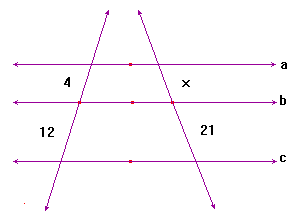
\includegraphics[scale=0.7]{figuras/fig46.png}
			\item 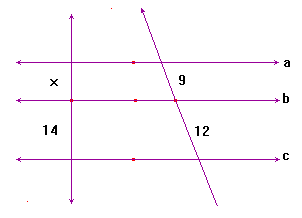
\includegraphics[scale=0.7]{figuras/fig47.png}
			\item 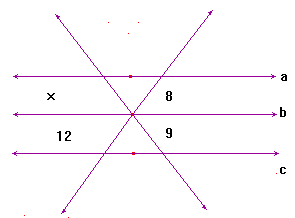
\includegraphics[scale=0.7]{figuras/fig48.png}
			\item 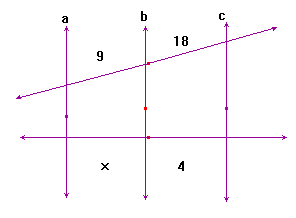
\includegraphics[scale=0.7]{figuras/fig49.png}
			\item 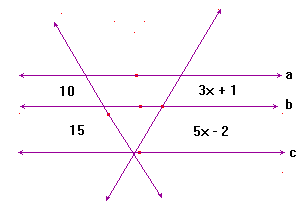
\includegraphics[scale=0.7]{figuras/fig50.png}
			\item 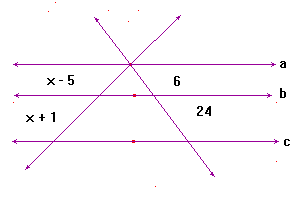
\includegraphics[scale=0.7]{figuras/fig51.png}
			\item 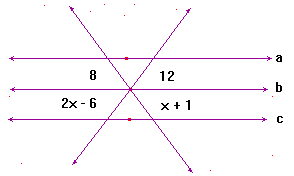
\includegraphics[scale=0.7]{figuras/fig52.png}
		\end{enumerate}
		\end{multicols}
		
	\item Determine x e y, sendo r, s, t e u retas paralelas.
		\begin{multicols}{2}
		\begin{enumerate}
			\item 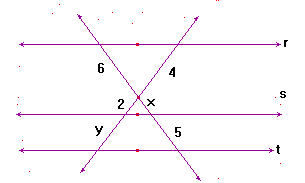
\includegraphics[scale=0.7]{figuras/fig53.png}
			\item 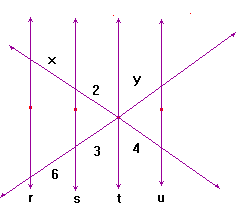
\includegraphics[scale=0.7]{figuras/fig54.png}
			\item 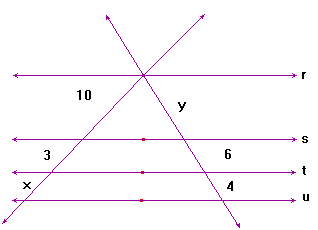
\includegraphics[scale=0.7]{figuras/fig55.png}
			\item 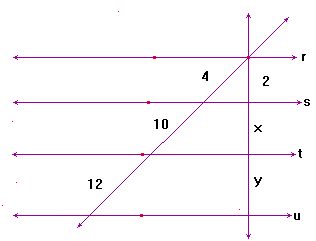
\includegraphics[scale=0.7]{figuras/fig56.png} 
		\end{enumerate}
		\end{multicols}
		
	\item Determine x e y, sendo r, s e t retas  paralelas.
	\begin{center}
	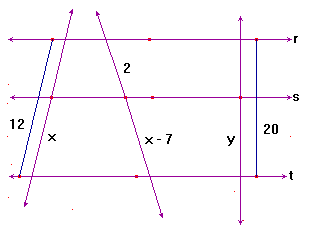
\includegraphics[scale=0.7]{figuras/fig57.png}
	\end{center}
	
	\item Uma reta paralela ao lado $\overline{BC}$ de um triângulo ABC determina o ponto D em $\overline{AB}$ e E em $\overline{AC}$. Sabendo-se que $\overline{AD}= x$, $\overline{BD} = x + 6$,  $\overline{AE} = 3$ e $\overline{EC} = 4$, determine o lado $\overline{AB}$ do triângulo.
	
	\item A figura abaixo indica três lotes de terreno com frente para a rua A e para rua B. as divisas dos lotes são perpendiculares à rua A. As frentes dos lotes 1, 2 e 3 para a rua A, medem, respectivamente, 15 m, 20 m e 25 m. A frente do lote 2 para a rua B mede 28 m. Qual é a medida da frente para a rua B dos lotes 1 e 3?
	\begin{center}
	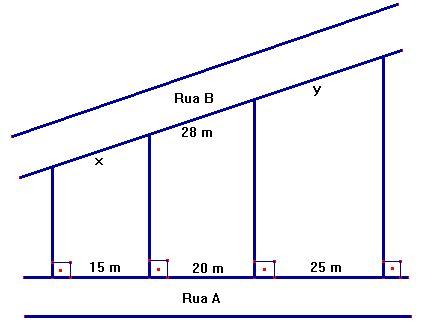
\includegraphics[scale=0.7]{figuras/fig58.png}
	\end{center}
	
	\item Um  feixe de quatro retas paralelas determina sobre uma transversal três segmentos consecutivos, que medem 5 cm, 6 cm e 9 cm. Calcule os comprimentos dos segmentos determinados pelo feixe em outra transversal, sabendo que o segmento desta, compreendido entre a primeira e a quarta paralela, mede 60 cm.
	
	\item As alturas de dois postes estão entre si assim como 3 esta para 5. Sabendo que o menor deles mede 6 m, então o maior mede:
	
	\item A figura abaixo nos mostra duas avenidas que partem de um mesmo ponto A e cortam duas ruas paralelas. Na primeira avenida, os quarteirões determinados pelas ruas paralelas tem 80 m e 90 m de comprimento, respectivamente. Na segunda avenida, um dos quarteirões determinados mede 60 m. Qual o comprimento do outro quarteirão?
	\begin{center}
	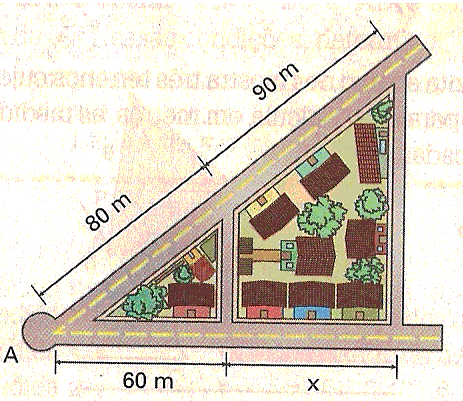
\includegraphics[scale=0.5]{figuras/fig59.png}
	\end{center}
	
	\item Na figura abaixo, sabe-se que $\overline{RS}//\overline{DE}$ e que $\overline{AE} = 42 cm$. Nessas condições, determine as medidas x  e y indicadas.
	\begin{center}
	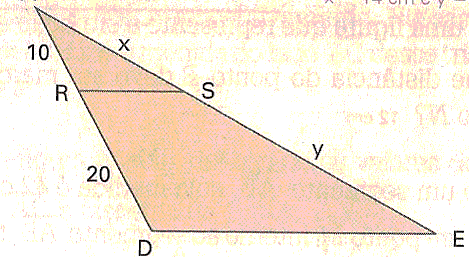
\includegraphics[scale=0.5]{figuras/fig60.png}
	\end{center}
	
	\item Num triângulo ABC, o lado $\overline{AB}$ mede 24 cm. Por um ponto D, sobre o lado $\overline{AB}$, distante 10 cm do vértice A, traça-se a paralela ao lado $\overline{BC}$, que corta o lado $\overline{AC}$ no ponto E e $\overline{AE}$ tem 15 cm, determine a medida do lado $\overline{AC}$.
	
	\item No triângulo ABC da figura, sabe-se que $\overline{DE} // \overline{BC}$. Calcule as medidas dos lados $\overline{AB}$ e $\overline{AC}$ do triângulo.
	\begin{center}
	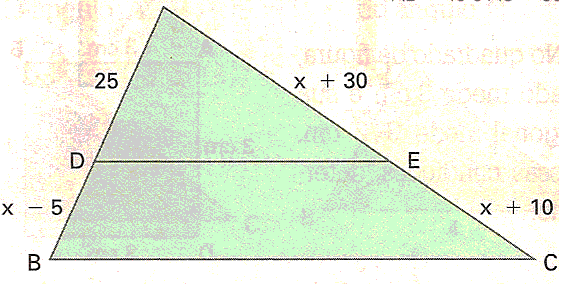
\includegraphics[scale=0.5]{figuras/fig61.png}
	\end{center}
	
	\item Na figura abaixo, $\overline{AE} // \overline{BD}$. Nessas condições, determine os valores de a e b.
	\begin{center}
	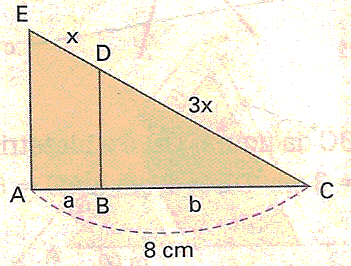
\includegraphics[scale=0.5]{figuras/fig62.png}
	\end{center}
	
	\item A planta abaixo no mostra três terrenos cujas laterais são paralelas. Calcule, em metros, as medidas x, y e z indicadas.
	\begin{center}
	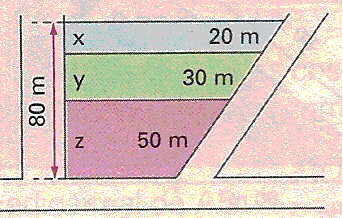
\includegraphics[scale=0.5]{figuras/fig63.png}
	\end{center}
	
	\item Dois postes perpendiculares ao solo estão a uma distância de 4 m um do outro, e um fio bem esticado de 5 m liga seus topos, como mostra a figura abaixo. Prolongando esse fio até prende-lo no solo, são utilizados mais 4 m de fio. Determine a distância entre o ponto onde o fio foi preso ao solo e o poste mais próximo a ele.
	\begin{center}
	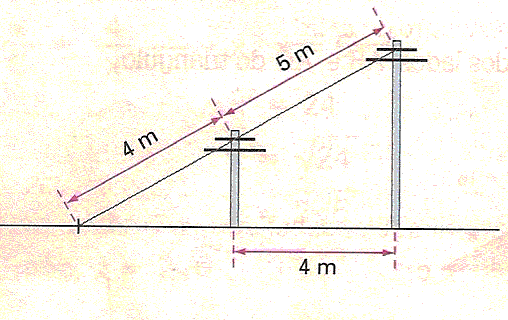
\includegraphics[scale=0.5]{figuras/fig64.png}
	\end{center}
	
	\item No triângulo abaixo, sabe-se que $\overline{DE} // \overline{BC}$. Calcule as medidas dos lados  $\overline{AB}$ e $\overline{AC}$ do triângulo.
	\begin{center}
	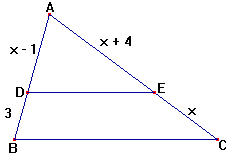
\includegraphics[scale=0.7]{figuras/fig65.png}
	\end{center}
	
	\item Em um triângulo retângulo, a hipotenusa mede 14 cm e um dos catetos mede $5\sqrt{3}$cm. Determine a medida do outro cateto.
\end{list}